\documentclass[11pt]{article}

% ---------------- Packages ----------------
\usepackage[letterpaper,margin=0.85in]{geometry}
\usepackage{amsmath,amssymb}
\usepackage[dvipsnames]{xcolor}
\usepackage{enumitem}
\usepackage{titlesec}
\usepackage{tikz}
\usepackage{mdframed}
\usepackage{fancyhdr}
\usepackage{parskip}

% ---------------- Colors ----------------
\definecolor{FangBlue}{HTML}{1F4E79}
\definecolor{FangAccent}{HTML}{C0392B}
\definecolor{FangGreen}{HTML}{1E8449}
\definecolor{FangOrange}{HTML}{B9770E}
\definecolor{RuleGray}{HTML}{6B7280}

% ---------------- Section styling ----------------
\titleformat{\section}
  {\color{FangBlue}\large\bfseries}{}{0pt}
  {\colorbox{FangBlue}{\textcolor{white}{\ \thesection\ }}\quad}
\titlespacing*{\section}{0pt}{1.5em}{0.7em}
\titleformat{\subsection}[runin]
  {\color{FangBlue}\bfseries}{}{0pt}{}[\ ]
\renewcommand{\thesection}{Topic \arabic{section}}

% ---------------- Header / footer ----------------
\pagestyle{fancy}
\fancyhf{}
\renewcommand{\headrulewidth}{0.4pt}
\lhead{\small\color{RuleGray}FangMath $\cdot$ Algebra 2 Practice}
\rhead{\small\color{RuleGray}Name: \underline{\hspace{3.2cm}}}
\cfoot{\small\color{RuleGray}\thepage}

% ---------------- Boxes ----------------
\newmdenv[linecolor=FangBlue,linewidth=0.8pt,roundcorner=5pt,
  backgroundcolor=FangBlue!5,innertopmargin=7pt,innerbottommargin=7pt,
  innerleftmargin=9pt,innerrightmargin=9pt,skipabove=6pt,skipbelow=8pt]{summary}
\newmdenv[linecolor=FangAccent!70,linewidth=0.8pt,roundcorner=5pt,
  backgroundcolor=FangAccent!4,innertopmargin=7pt,innerbottommargin=7pt,
  innerleftmargin=9pt,innerrightmargin=9pt,skipabove=6pt,skipbelow=8pt]{example}

% ---------------- Difficulty badges ----------------
\newcommand{\easy}{{\small\color{FangGreen}\textbf{(Easy)}}}
\newcommand{\med}{{\small\color{FangOrange}\textbf{(Medium)}}}
\newcommand{\hard}{{\small\color{FangAccent}\textbf{(Hard)}}}

% ---------------- Practice list environment ----------------
\newlist{practice}{enumerate}{1}
\setlist[practice]{label=\textbf{\arabic*.},leftmargin=2em,itemsep=10pt,topsep=4pt}

% ---------------- Coordinate grid helpers ----------------
% Blank grid for students
\newcommand{\blankgrid}{%
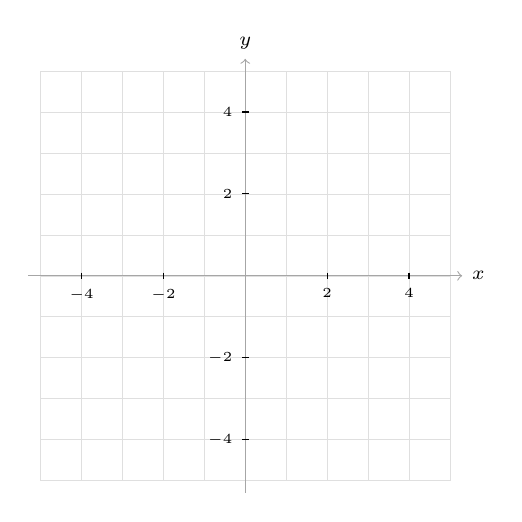
\begin{tikzpicture}[scale=0.52,baseline=0pt]
  \draw[step=1,gray!25,very thin] (-5,-5) grid (5,5);
  \draw[->,gray!70] (-5.3,0)--(5.3,0) node[right,black]{\scriptsize$x$};
  \draw[->,gray!70] (0,-5.3)--(0,5.3) node[above,black]{\scriptsize$y$};
  \foreach \i in {-4,-2,2,4}{%
    \draw (\i,0.08)--(\i,-0.08) node[below,black]{\tiny$\i$};
    \draw (0.08,\i)--(-0.08,\i) node[left,black]{\tiny$\i$};}
\end{tikzpicture}}

% Axes drawing used inside answer-key figures (call at top, unclipped)
\newcommand{\axesbg}{%
  \draw[step=1,gray!25,very thin] (-5,-5) grid (5,5);
  \draw[->,gray!70] (-5.3,0)--(5.3,0) node[right,black]{\scriptsize$x$};
  \draw[->,gray!70] (0,-5.3)--(0,5.3) node[above,black]{\scriptsize$y$};
  \foreach \i in {-4,-2,2,4}{%
    \draw (\i,0.08)--(\i,-0.08) node[below,black]{\tiny$\i$};
    \draw (0.08,\i)--(-0.08,\i) node[left,black]{\tiny$\i$};}}

\newcommand{\opendot}[2]{\draw[FangBlue,thick,fill=white] (#1,#2) circle (0.13);}
\newcommand{\closeddot}[2]{\fill[FangBlue] (#1,#2) circle (0.13);}

\begin{document}

% ==================== TITLE ====================
\begin{center}
  {\color{FangBlue}\Huge\bfseries Algebra 2 --- Practice Worksheet}\\[3pt]
  {\color{RuleGray}\large Sequences \,$\cdot$\, Functions \,$\cdot$\, Systems \,$\cdot$\, Rational Expressions}\\[6pt]
  {\small\color{RuleGray}Name: \underline{\hspace{5cm}} \qquad Date: \underline{\hspace{3.5cm}}}
\end{center}
\vspace{2pt}

\begin{summary}
\textbf{How this packet is organized.} Seven topics grouped into four parts.
Each topic has a short \textbf{Summary}, one or two worked \textbf{Examples}, and \textbf{5 practice
problems} rising in difficulty: \easy\ (1) $\rightarrow$ \med\ (2) $\rightarrow$ \hard\ (2).
\textbf{Full worked solutions are in the Answer Key at the end.}

\smallskip
\textbf{Part I --- Sequences:} Topic 1. \quad
\textbf{Part II --- Functions:} Topic 2. \quad
\textbf{Part III --- Systems:} Topics 3--4. \quad
\textbf{Part IV --- Rational \& Radical Expressions and Equations:} Topics 5--7.
\end{summary}

% ============================================================
% TOPIC 1 — ARITHMETIC SEQUENCES
% ============================================================
\section{Arithmetic Sequences}

\begin{summary}
An \textbf{arithmetic sequence} is a list of numbers with a \textbf{constant common difference} $d$
between consecutive terms.
\[
d = a_n - a_{n-1}\qquad(\text{same gap every step})
\]
The \textbf{$n$-th term formula} lets you jump straight to any term without listing them all:
\[
\boxed{\,a_n = a_1 + (n-1)\,d\,}
\]
where $a_1$ is the first term and $n$ is the term number.
\textbf{Two useful moves:} (1) find a specific term by plugging in $n$;
(2) find $d$ and $a_1$ from two known terms, then build the formula.
\end{summary}

\begin{example}
\textbf{Example 1 (find a term).} If $a_1 = 3$ and $d = 5$, find $a_{10}$.\\
$a_{10} = 3 + (10-1)(5) = 3 + 45 = 48.$

\smallskip
\textbf{Example 2 (build the formula).} For $7,\,11,\,15,\,19,\dots$:
$d = 4,\ a_1 = 7$, so $a_n = 7 + (n-1)(4) = 4n + 3$. Then $a_{20} = 4(20)+3 = 83.$

\smallskip
\textbf{Example 3 (from two terms).} If $a_4 = 14$ and $a_9 = 34$:
subtract to get $a_9 - a_4 = 5d \Rightarrow 20 = 5d \Rightarrow d = 4$;
then $a_1 = a_4 - 3d = 14 - 12 = 2$, so $a_n = 2 + (n-1)(4)=4n-2.$
\end{example}

\textbf{Practice}
\begin{practice}
  \item \easy\ \ Given $a_1 = 5$ and $d = 3$, find $a_8$.
  \item \med\ \ Write the $n$-th term formula for $12,\,9,\,6,\,3,\dots$ and then find $a_{15}$.
  \item \med\ \ In an arithmetic sequence $a_1 = -4$ and $a_{12} = 29$. Find the common difference $d$ and the value of $a_{20}$.
  \item \hard\ \ The $5$th term of a sequence is $22$ and the $11$th term is $52$. Write the $n$-th term formula and find $a_{30}$.
  \item \hard\ \ How many terms are in the arithmetic sequence $4,\,10,\,16,\,\dots,\,106$?
\end{practice}

% ============================================================
% TOPIC 2 — PIECEWISE FUNCTIONS
% ============================================================
\section{Piecewise Functions}

\begin{summary}
A \textbf{piecewise function} uses \textbf{different rules on different parts of the domain}. For example
\[
f(x)=\begin{cases}
2x+1, & x<0\\[2pt]
x^2, & x\ge 0
\end{cases}
\]
\textbf{To evaluate:} decide which interval the input falls in, then use that piece's rule.\\
\textbf{To graph:} graph each piece \emph{only} over its interval. Use an \textbf{open circle} $\circ$ at an
endpoint with a strict inequality ($<$ or $>$) and a \textbf{closed dot} $\bullet$ with $\le$ or $\ge$.\\
\textbf{To write a piecewise rule from a graph:} find each straight piece's equation ($y=mx+b$) and the
$x$-interval it covers; note which endpoints are open vs.\ closed.
\end{summary}

\begin{example}
\textbf{Example (evaluate).} For the $f$ above:
$f(-2)=2(-2)+1=-3$ (used the top piece since $-2<0$); \ $f(3)=3^2=9$ (bottom piece since $3\ge 0$).

\smallskip
\textbf{Example (graph).} $g(x)=\begin{cases}-x+2,& x\le 1\\ 3,& x>1\end{cases}$ is a line of slope $-1$ up to a
\emph{closed} dot at $(1,1)$, then a horizontal ray at height $3$ starting with an \emph{open} circle at $(1,3)$.
\end{example}

\textbf{Practice}
\begin{practice}
  \item \easy\ \ Let $f(x)=\begin{cases}x+4, & x<2\\ 2x, & x\ge 2\end{cases}$\ \ Find $f(-1)$, $f(2)$, and $f(5)$.
  \item \med\ \ Graph \ $f(x)=\begin{cases}x+1, & x<1\\ 4-x, & x\ge 1\end{cases}$ \ on the grid. Mark open/closed endpoints.\\[4pt]
        \blankgrid
  \item \med\ \ Write the piecewise function shown in the graph.\\[4pt]
        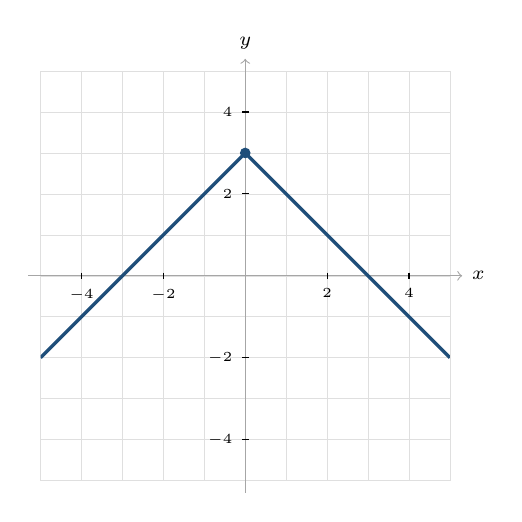
\begin{tikzpicture}[scale=0.52,baseline=0pt]
          \axesbg
          \begin{scope}\clip(-5,-5) rectangle (5,5);
            \draw[FangBlue,very thick] (-5,-2)--(0,3);   % y=x+3, x<=0
            \draw[FangBlue,very thick] (0,3)--(5,-2);     % y=-x+3, x>0
          \end{scope}
          \closeddot{0}{3}
        \end{tikzpicture}
  \item \hard\ \ Graph \ $f(x)=\begin{cases}x+2, & x<0\\ 1, & 0\le x\le 2\\ -x+4, & x>2\end{cases}$ and state the \textbf{range}.\\[4pt]
        \blankgrid
  \item \hard\ \ A rideshare charges a \$4 base fare plus \$2 per mile for the first $5$ miles, then \$1.50 per mile
        after that. Write a piecewise function $C(x)$ for the total cost of an $x$-mile trip, then find $C(3)$ and $C(8)$.
\end{practice}

% ============================================================
% TOPIC 3 — SYSTEMS OF LINEAR EQUATIONS
% ============================================================
\section{Systems of Linear Equations}

\begin{summary}
A \textbf{system} is two equations that must be true at the same time; the \textbf{solution} $(x,y)$ is the point
that satisfies both. Three algebraic tools:
\begin{itemize}[leftmargin=1.4em,itemsep=1pt,topsep=2pt]
  \item \textbf{Substitution:} solve one equation for a variable, then substitute into the other.
  \item \textbf{Elimination:} add or subtract multiples of the equations to cancel one variable.
  \item \textbf{Graphing:} the intersection point is the solution.
\end{itemize}
\textbf{Outcomes:} one solution (lines cross), \textbf{no solution} (parallel lines), or
\textbf{infinitely many} (same line).
\end{summary}

\begin{example}
\textbf{Example (substitution).} $y = 2x-1$ and $3x + y = 9$. Substitute:
$3x + (2x-1) = 9 \Rightarrow 5x = 10 \Rightarrow x = 2$, so $y = 3$. Solution $(2,3)$.

\smallskip
\textbf{Example (elimination).} $2x+3y=12$ and $2x-y=4$. Subtract the equations:
$4y = 8 \Rightarrow y = 2$; back-substitute $2x - 2 = 4 \Rightarrow x = 3$. Solution $(3,2)$.
\end{example}

\textbf{Practice}
\begin{practice}
  \item \easy\ \ Solve by substitution: \ $y = x+2,\quad 3x + y = 10.$
  \item \med\ \ Solve by elimination: \ $3x + 2y = 16,\quad x - 2y = -8.$
  \item \med\ \ Solve: \ $4x + 3y = 10,\quad 2x - y = 0.$
  \item \hard\ \ Solve: \ $3x + 4y = -1,\quad 5x + 6y = 1.$
  \item \hard\ \ A theater sells adult tickets for \$12 and child tickets for \$8. One night they sold $200$
        tickets and collected \$2080. How many of each type were sold? (Set up and solve a system.)
\end{practice}

% ============================================================
% TOPIC 4 — SYSTEMS OF LINEAR INEQUALITIES
% ============================================================
\section{Graphing Systems of Linear Inequalities}

\begin{summary}
To graph a system of inequalities, graph each one and take the \textbf{overlap}:
\begin{itemize}[leftmargin=1.4em,itemsep=1pt,topsep=2pt]
  \item Draw the boundary line: \textbf{solid} for $\le$ or $\ge$, \textbf{dashed} for $<$ or $>$.
  \item Shade the correct side. \textbf{Test a point} not on the line (often the origin): if it makes the
        inequality true, shade that side; if false, shade the other side.
  \item The \textbf{solution set} is the region where \emph{all} shadings overlap.
\end{itemize}
\end{summary}

\begin{example}
\textbf{Example.} For $y \ge x-1$ (solid line, shade above) and $y < -x+3$ (dashed line, shade below), the
solution is the wedge where the two shaded regions overlap. Testing $(0,0)$: $0\ge -1$ \checkmark\ and
$0 < 3$ \checkmark, so $(0,0)$ lies in the solution.
\end{example}

\textbf{Practice} \ (Graph each system; shade the solution region.)
\begin{practice}
  \item \easy\ \ $y \ge 1$ \ and \ $x \le 3$.\\[4pt]
        \blankgrid
  \item \med\ \ $y < x+2$ \ and \ $y \ge -x$.\\[4pt]
        \blankgrid
  \item \med\ \ $y \ge 2x-3$ \ and \ $y < -x+4$.\\[4pt]
        \blankgrid
  \item \hard\ \ $y \le -x+5$, \ $y \ge x-1$, \ and \ $x \ge 0$ \ (three inequalities).\\[4pt]
        \blankgrid
  \item \hard\ \ $2x + y < 4$ \ and \ $y \ge \tfrac{1}{2}x - 2$. \ Then state whether $(0,0)$ is a solution.\\[4pt]
        \blankgrid
\end{practice}

% ============================================================
% TOPIC 5 — RATIONAL EXPONENTS
% ============================================================
\section{Evaluating Expressions with Rational Exponents}

\begin{summary}
A \textbf{rational exponent} means a root. The denominator is the root; the numerator is the power:
\[
a^{1/n} = \sqrt[n]{a}, \qquad
\boxed{\,a^{m/n} = \left(\sqrt[n]{a}\right)^{m} = \sqrt[n]{a^{m}}\,}
\]
A \textbf{negative} rational exponent means take the reciprocal:
\[
a^{-m/n} = \frac{1}{a^{m/n}}.
\]
\textbf{Best strategy for numbers:} take the \emph{root first} (numbers stay small), then apply the power.
\end{summary}

\begin{example}
\textbf{Example 1.} $27^{1/3} = \sqrt[3]{27} = 3.$

\smallskip
\textbf{Example 2.} $16^{3/4} = \left(16^{1/4}\right)^{3} = 2^{3} = 8.$

\smallskip
\textbf{Example 3 (negative).} $8^{-2/3} = \dfrac{1}{8^{2/3}} = \dfrac{1}{\left(8^{1/3}\right)^{2}}
= \dfrac{1}{2^{2}} = \dfrac{1}{4}.$
\end{example}

\textbf{Practice} \ (Evaluate; give exact values.)
\begin{practice}
  \item \easy\ \ $25^{1/2}$
  \item \med\ \ $8^{4/3}$
  \item \med\ \ $81^{3/4}$
  \item \hard\ \ $32^{-3/5}$
  \item \hard\ \ $\left(\dfrac{27}{8}\right)^{-2/3}$
\end{practice}

% ============================================================
% TOPIC 6 — RATIONAL EQUATIONS
% ============================================================
\section{Solving Rational Equations}

\begin{summary}
A \textbf{rational equation} has one or more variables in a denominator. To solve:
\begin{enumerate}[leftmargin=1.5em,itemsep=1pt,topsep=2pt]
  \item Find the \textbf{LCD} (least common denominator) of all fractions.
  \item Multiply \emph{every} term by the LCD to clear the denominators.
  \item Solve the resulting equation (it may be linear or quadratic).
  \item \textbf{Check for extraneous solutions:} any answer that makes a denominator $0$ is rejected.
\end{enumerate}
For a simple proportion $\dfrac{A}{B}=\dfrac{C}{D}$, you may \textbf{cross-multiply}: $AD = BC$.
\end{summary}

\begin{example}
\textbf{Example 1.} $\dfrac{x}{3} + \dfrac{1}{2} = \dfrac{5}{6}$. Multiply every term by $6$:
$2x + 3 = 5 \Rightarrow 2x = 2 \Rightarrow x = 1.$

\smallskip
\textbf{Example 2 (extraneous).} $\dfrac{x}{x-3} = \dfrac{3}{x-3} + 4$. Multiply by $(x-3)$:
$x = 3 + 4(x-3) \Rightarrow x = 3$. But $x=3$ makes a denominator $0$, so it is \textbf{rejected}:
\emph{no solution.}
\end{example}

\textbf{Practice}
\begin{practice}
  \item \easy\ \ $\dfrac{x}{4} + \dfrac{1}{2} = \dfrac{5}{4}$
  \item \med\ \ $\dfrac{5}{x} = \dfrac{10}{x+3}$
  \item \med\ \ $\dfrac{2}{x-1} + 3 = \dfrac{5}{x-1}$
  \item \hard\ \ $\dfrac{12}{x} = x + 4$
  \item \hard\ \ $\dfrac{x}{x-3} = \dfrac{3}{x-3} + 4$
\end{practice}

% ============================================================
% TOPIC 7 — RADICAL (ROOT) EQUATIONS
% ============================================================
\section{Solving Radical (Root) Equations}

\begin{summary}
A \textbf{radical equation} has a variable \textbf{under a radical} (usually a square root). To solve:
\begin{enumerate}[leftmargin=1.5em,itemsep=1pt,topsep=2pt]
  \item \textbf{Isolate the radical} on one side of the equation.
  \item \textbf{Undo the root} by raising both sides to the matching power (square a square root, cube a cube root).
  \item Solve the resulting equation (it may be linear or quadratic).
  \item \textbf{Check every answer in the original equation.} Squaring can create \emph{extraneous}
        solutions --- values that satisfy the squared equation but not the original one.
\end{enumerate}
Key fact: $\left(\sqrt{a}\right)^{2} = a$, so squaring removes a square root --- but only \emph{after} it is alone.
\end{summary}

\begin{example}
\textbf{Example 1.} $\sqrt{x+3} = 4$. Square both sides: $x + 3 = 16 \Rightarrow x = 13.$
\ Check: $\sqrt{16} = 4$ \checkmark.

\smallskip
\textbf{Example 2 (isolate first).} $\sqrt{2x-1} + 3 = 8$. Isolate: $\sqrt{2x-1} = 5$; square:
$2x - 1 = 25 \Rightarrow x = 13.$

\smallskip
\textbf{Example 3 (extraneous).} $\sqrt{x+2} = x$. Square: $x + 2 = x^{2} \Rightarrow x^{2} - x - 2 = 0
\Rightarrow (x-2)(x+1) = 0.$ Candidates $x = 2,\,-1$. Check: $x=2$ gives $\sqrt{4}=2$ \checkmark;\
$x=-1$ gives $\sqrt{1}=1 \neq -1$ \textbf{\color{FangAccent}(reject)}. \ Only $x = 2.$
\end{example}

\textbf{Practice}
\begin{practice}
  \item \easy\ \ $\sqrt{x} = 7$
  \item \med\ \ $\sqrt{x - 4} = 6$
  \item \med\ \ $\sqrt{3x + 1} - 2 = 3$
  \item \hard\ \ $\sqrt{x + 6} = x$
  \item \hard\ \ The time (in seconds) for an object to fall $d$ feet is modeled by $t = \sqrt{\dfrac{d}{16}}$.
        If a stone falls for $2.5$ seconds before it hits the ground, how far did it fall?
\end{practice}

% ============================================================
% ANSWER KEY
% ============================================================
\clearpage
\begin{center}
  {\color{FangAccent}\Huge\bfseries Answer Key}\\[2pt]
  {\small\color{RuleGray}Full worked solutions}
\end{center}
\vspace{4pt}

% ---- Topic 1 ----
\subsection*{\color{FangBlue}Topic 1 --- Arithmetic Sequences}
\begin{enumerate}[leftmargin=2em,itemsep=6pt]
  \item $a_8 = a_1 + 7d = 5 + 7(3) = \boxed{26}.$
  \item $d = 9 - 12 = -3,\ a_1 = 12$, so $a_n = 12 + (n-1)(-3) = \boxed{-3n + 15}.$
        Then $a_{15} = -3(15)+15 = \boxed{-30}.$
  \item $a_{12} = a_1 + 11d \Rightarrow -4 + 11d = 29 \Rightarrow 11d = 33 \Rightarrow \boxed{d = 3}.$
        \ Then $a_{20} = -4 + 19(3) = \boxed{53}.$
  \item $a_{11} - a_5 = 6d \Rightarrow 52 - 22 = 30 \Rightarrow d = 5.$
        \ $a_1 = a_5 - 4d = 22 - 20 = 2$, so $a_n = 2 + (n-1)(5) = \boxed{5n - 3}.$
        \ Then $a_{30} = 5(30) - 3 = \boxed{147}.$
  \item Here $a_1 = 4,\ d = 6$, so $a_n = 4 + (n-1)(6) = 6n - 2.$
        Set $6n - 2 = 106 \Rightarrow 6n = 108 \Rightarrow n = \boxed{18}$ terms.
\end{enumerate}

% ---- Topic 2 ----
\subsection*{\color{FangBlue}Topic 2 --- Piecewise Functions}
\begin{enumerate}[leftmargin=2em,itemsep=8pt]
  \item $f(-1)=(-1)+4=\boxed{3}$ (since $-1<2$); \ $f(2)=2(2)=\boxed{4}$ (since $2\ge 2$);
        \ $f(5)=2(5)=\boxed{10}.$
  \item Line $y=x+1$ for $x<1$ ends at an \emph{open} circle $(1,2)$; ray $y=4-x$ for $x\ge 1$ starts at a
        \emph{closed} dot $(1,3)$ — a jump at $x=1$.\\[3pt]
        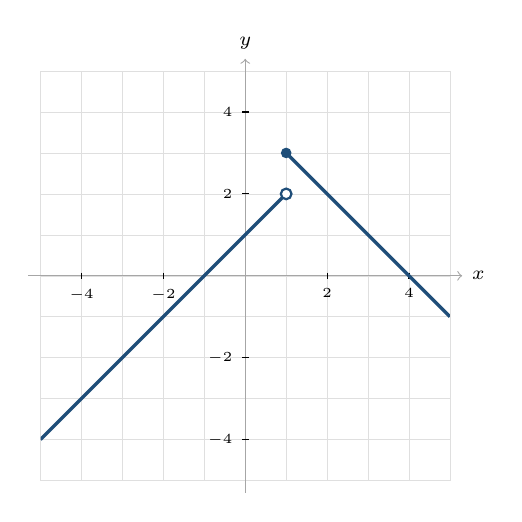
\begin{tikzpicture}[scale=0.52,baseline=0pt]
          \axesbg
          \begin{scope}\clip(-5,-5) rectangle (5,5);
            \draw[FangBlue,very thick] (-5,-4)--(1,2);
            \draw[FangBlue,very thick] (1,3)--(5,-1);
          \end{scope}
          \opendot{1}{2}\closeddot{1}{3}
        \end{tikzpicture}
  \item Left piece has slope $+1$ through $(0,3)$: $y = x+3$ for $x\le 0$.
        Right piece has slope $-1$ through $(0,3)$: $y = -x+3$ for $x>0$. So
        \[
          f(x)=\begin{cases}x+3, & x\le 0\\ -x+3, & x>0\end{cases}
        \]
  \item Endpoints: open $(0,2)$ \& closed $(0,1)$ at $x=0$; closed $(2,1)$ \& open $(2,2)$ at $x=2$.
        \textbf{Range: } $(-\infty,\,2)$.\\[3pt]
        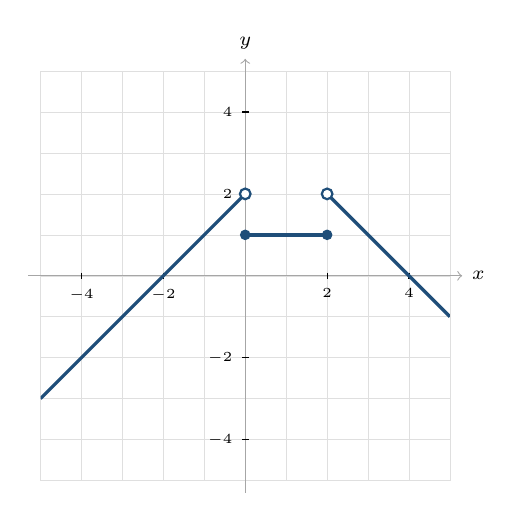
\begin{tikzpicture}[scale=0.52,baseline=0pt]
          \axesbg
          \begin{scope}\clip(-5,-5) rectangle (5,5);
            \draw[FangBlue,very thick] (-5,-3)--(0,2);   % x+2, x<0
            \draw[FangBlue,very thick] (0,1)--(2,1);      % 1, 0<=x<=2
            \draw[FangBlue,very thick] (2,2)--(5,-1);     % -x+4, x>2
          \end{scope}
          \opendot{0}{2}\closeddot{0}{1}\closeddot{2}{1}\opendot{2}{2}
        \end{tikzpicture}
  \item First $5$ miles cost $4 + 2x$; at $5$ miles that is \$14, and each extra mile adds \$1.50:
        \[
          C(x)=\begin{cases}4 + 2x, & 0\le x\le 5\\[2pt] 1.5x + 6.5, & x > 5\end{cases}
        \]
        $C(3) = 4 + 2(3) = \boxed{\$10}$; \ $C(8) = 1.5(8) + 6.5 = 12 + 6.5 = \boxed{\$18.50}.$
\end{enumerate}

% ---- Topic 3 ----
\subsection*{\color{FangBlue}Topic 3 --- Systems of Linear Equations}
\begin{enumerate}[leftmargin=2em,itemsep=6pt]
  \item Substitute $y=x+2$: \ $3x + (x+2) = 10 \Rightarrow 4x = 8 \Rightarrow x = 2$, \ $y = 4.$
        \ Solution $\boxed{(2,4)}.$
  \item Add the equations: $(3x+2y)+(x-2y) = 16 + (-8) \Rightarrow 4x = 8 \Rightarrow x = 2.$
        \ Then $2 - 2y = -8 \Rightarrow y = 5.$ \ Solution $\boxed{(2,5)}.$
  \item From the second equation $y = 2x$. Substitute: $4x + 3(2x) = 10 \Rightarrow 10x = 10 \Rightarrow x = 1$,
        \ $y = 2.$ \ Solution $\boxed{(1,2)}.$
  \item Multiply the first by $3$ and the second by $2$: $9x+12y=-3$ and $10x+12y=2.$
        Subtract: $-x = -5 \Rightarrow x = 5.$ Then $3(5)+4y=-1 \Rightarrow 4y = -16 \Rightarrow y = -4.$
        \ Solution $\boxed{(5,-4)}.$
  \item Let $a=$ adult, $c=$ child. \ $a + c = 200$ and $12a + 8c = 2080.$
        Substitute $c = 200 - a$: \ $12a + 8(200 - a) = 2080 \Rightarrow 4a = 480 \Rightarrow a = 120.$
        Then $c = 80.$ \ $\boxed{120 \text{ adult},\ 80 \text{ child}}.$
\end{enumerate}

% ---- Topic 4 ----
\subsection*{\color{FangBlue}Topic 4 --- Systems of Linear Inequalities}
Shaded region $=$ solution set; dashed $=$ strict ($<,>$), solid $=$ inclusive ($\le,\ge$).

\vspace{4pt}
\begin{enumerate}[leftmargin=2em,itemsep=10pt]
  \item $y \ge 1$ (solid, shade up) and $x \le 3$ (solid, shade left). Overlap: the region at/above $y=1$ and
        at/left of $x=3$.\\[3pt]
        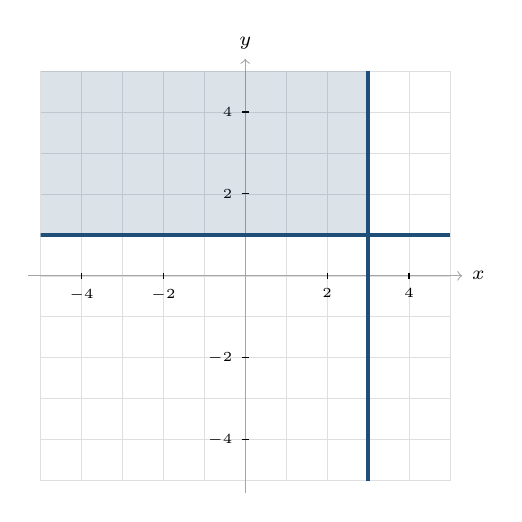
\begin{tikzpicture}[scale=0.52,baseline=0pt]
          \axesbg
          \begin{scope}\clip(-5,-5) rectangle (5,5);
            \fill[FangBlue,opacity=0.16] (-5,1) rectangle (3,5);
            \draw[FangBlue,very thick] (-6,1)--(6,1);
            \draw[FangBlue,very thick] (3,-6)--(3,6);
          \end{scope}
        \end{tikzpicture}
  \item $y<x+2$ (dashed, shade below) and $y\ge -x$ (solid, shade above); lines meet at $(-1,1)$.
        Overlap opens to the right.\\[3pt]
        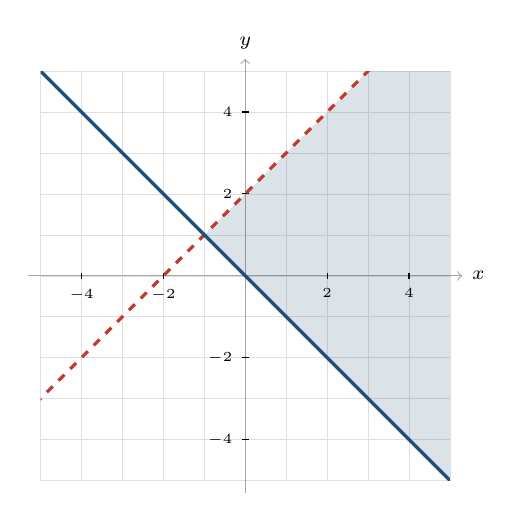
\begin{tikzpicture}[scale=0.52,baseline=0pt]
          \axesbg
          \begin{scope}\clip(-5,-5) rectangle (5,5);
            \fill[FangBlue,opacity=0.16] (-1,1)--(3,5)--(5,5)--(5,-5)--cycle;
            \draw[FangAccent,very thick,dashed] (-8,-6)--(6,8);   % y=x+2
            \draw[FangBlue,very thick] (-6,6)--(6,-6);            % y=-x
          \end{scope}
        \end{tikzpicture}
  \item $y\ge 2x-3$ (solid, shade above) and $y<-x+4$ (dashed, shade below); lines meet at
        $\left(\tfrac{7}{3},\tfrac{5}{3}\right)$. Overlap opens to the left.\\[3pt]
        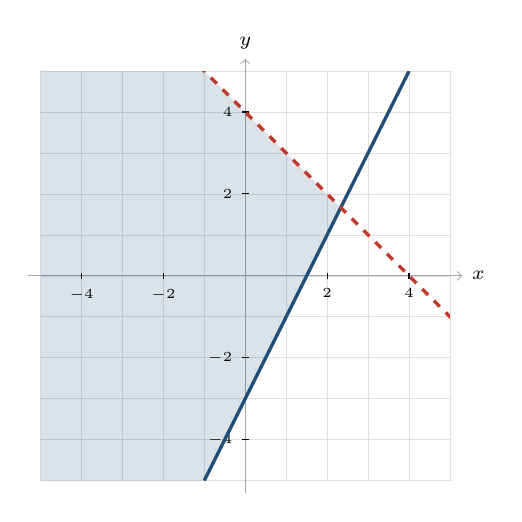
\begin{tikzpicture}[scale=0.52,baseline=0pt]
          \axesbg
          \begin{scope}\clip(-5,-5) rectangle (5,5);
            \fill[FangBlue,opacity=0.16] (2.333,1.667)--(-1,-5)--(-5,-5)--(-5,5)--(-1,5)--cycle;
            \draw[FangBlue,very thick] (-1,-5)--(4,5);            % y=2x-3
            \draw[FangAccent,very thick,dashed] (-6,10)--(9,-5);  % y=-x+4
          \end{scope}
        \end{tikzpicture}
  \item $y\le -x+5$ (solid), $y\ge x-1$ (solid), $x\ge 0$ (solid). Overlap is the triangle with vertices
        $(0,-1),\ (0,5),\ (3,2)$.\\[3pt]
        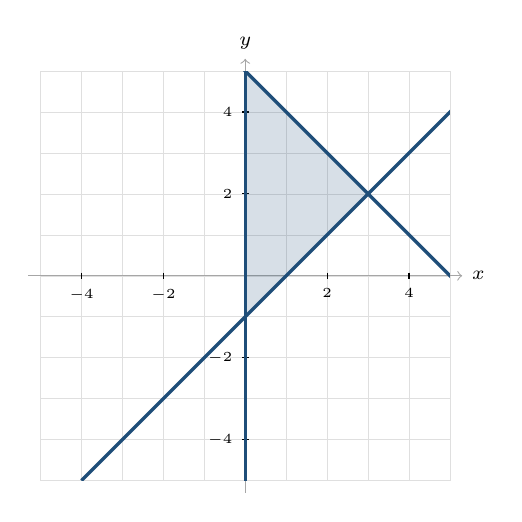
\begin{tikzpicture}[scale=0.52,baseline=0pt]
          \axesbg
          \begin{scope}\clip(-5,-5) rectangle (5,5);
            \fill[FangBlue,opacity=0.18] (0,-1)--(0,5)--(3,2)--cycle;
            \draw[FangBlue,very thick] (-1,6)--(6,-1);   % y=-x+5
            \draw[FangBlue,very thick] (-4,-5)--(6,5);   % y=x-1
            \draw[FangBlue,very thick] (0,-6)--(0,6);     % x=0
          \end{scope}
        \end{tikzpicture}
  \item Rewrite the first as $y<-2x+4$ (dashed, shade below); $y\ge\tfrac12 x-2$ (solid, shade above);
        lines meet at $(2.4,-0.8)$. \ Test $(0,0)$: $2(0)+0=0<4$ \checkmark\ and $0\ge -2$ \checkmark, so
        \textbf{$(0,0)$ IS a solution}.\\[3pt]
        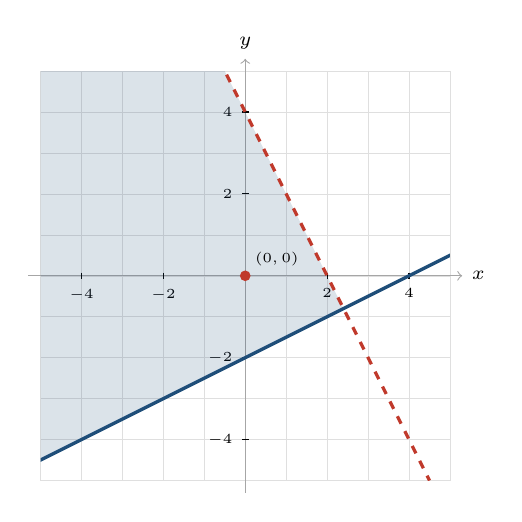
\begin{tikzpicture}[scale=0.52,baseline=0pt]
          \axesbg
          \begin{scope}\clip(-5,-5) rectangle (5,5);
            \fill[FangBlue,opacity=0.16] (2.4,-0.8)--(-5,-4.5)--(-5,5)--(-0.5,5)--cycle;
            \draw[FangAccent,very thick,dashed] (-1,6)--(4.5,-5);  % y=-2x+4
            \draw[FangBlue,very thick] (-6,-5)--(6,1);             % y=0.5x-2
            \fill[FangAccent] (0,0) circle (0.13) node[above right,black]{\tiny$(0,0)$};
          \end{scope}
        \end{tikzpicture}
\end{enumerate}

% ---- Topic 5 ----
\subsection*{\color{FangBlue}Topic 5 --- Rational Exponents}
\begin{enumerate}[leftmargin=2em,itemsep=6pt]
  \item $25^{1/2} = \sqrt{25} = \boxed{5}.$
  \item $8^{4/3} = \left(8^{1/3}\right)^{4} = 2^{4} = \boxed{16}.$
  \item $81^{3/4} = \left(81^{1/4}\right)^{3} = 3^{3} = \boxed{27}.$
  \item $32^{-3/5} = \dfrac{1}{32^{3/5}} = \dfrac{1}{\left(32^{1/5}\right)^{3}} = \dfrac{1}{2^{3}}
        = \boxed{\dfrac{1}{8}}.$
  \item $\left(\dfrac{27}{8}\right)^{-2/3} = \left(\dfrac{8}{27}\right)^{2/3}
        = \left(\left(\dfrac{8}{27}\right)^{1/3}\right)^{2} = \left(\dfrac{2}{3}\right)^{2}
        = \boxed{\dfrac{4}{9}}.$
\end{enumerate}

% ---- Topic 6 ----
\subsection*{\color{FangBlue}Topic 6 --- Rational Equations}
\begin{enumerate}[leftmargin=2em,itemsep=6pt]
  \item Multiply by $4$: \ $x + 2 = 5 \Rightarrow \boxed{x = 3}.$ \ ($x=3$ keeps no denominator $0$: valid.)
  \item Cross-multiply: \ $5(x+3) = 10x \Rightarrow 5x + 15 = 10x \Rightarrow 15 = 5x \Rightarrow \boxed{x = 3}.$
        \ (Need $x\neq 0,-3$: valid.)
  \item Multiply by $(x-1)$: \ $2 + 3(x-1) = 5 \Rightarrow 3x - 1 = 5 \Rightarrow 3x = 6 \Rightarrow \boxed{x = 2}.$
        \ (Need $x\neq 1$: valid.)
  \item Multiply by $x$: \ $12 = x^2 + 4x \Rightarrow x^2 + 4x - 12 = 0 \Rightarrow (x+6)(x-2) = 0.$
        \ So $\boxed{x = -6 \text{ or } x = 2}$ (both $\neq 0$: valid).
  \item Multiply by $(x-3)$: \ $x = 3 + 4(x-3) \Rightarrow x = 4x - 9 \Rightarrow x = 3.$
        But $x = 3$ makes $x-3 = 0$, so it is extraneous. \ \textbf{No solution.}
        \ (Equivalently: $\frac{x-3}{x-3} = 4 \Rightarrow 1 = 4$, a contradiction.)
\end{enumerate}

% ---- Topic 7 ----
\subsection*{\color{FangBlue}Topic 7 --- Radical (Root) Equations}
\begin{enumerate}[leftmargin=2em,itemsep=6pt]
  \item Square both sides: $x = 7^{2} = \boxed{49}.$ \ (Check: $\sqrt{49}=7$ \checkmark.)
  \item Square both sides: $x - 4 = 6^{2} = 36 \Rightarrow \boxed{x = 40}.$ \ (Check: $\sqrt{36}=6$ \checkmark.)
  \item Isolate the radical: $\sqrt{3x+1} = 5$; square: $3x + 1 = 25 \Rightarrow 3x = 24 \Rightarrow \boxed{x = 8}.$
        \ (Check: $\sqrt{25}-2 = 5-2 = 3$ \checkmark.)
  \item Square: $x + 6 = x^{2} \Rightarrow x^{2} - x - 6 = 0 \Rightarrow (x-3)(x+2) = 0.$
        \ Candidates $x = 3,\,-2$. Check: $x=3$ gives $\sqrt{9}=3$ \checkmark;\
        $x=-2$ gives $\sqrt{4}=2 \neq -2$ \textbf{\color{FangAccent}(reject)}. \ Only $\boxed{x = 3}.$
  \item Solve $2.5 = \sqrt{\dfrac{d}{16}}$. Square both sides: $6.25 = \dfrac{d}{16}
        \Rightarrow d = 6.25 \times 16 = \boxed{100 \text{ feet}}.$
\end{enumerate}

\vfill
\begin{center}
{\small\color{RuleGray}FangMath $\cdot$ \emph{Learn Math the Smart Way}}
\end{center}

\end{document}
